\documentclass[aspectratio=43,10pt]{beamer}

% =============================================================================
% PPD-II SECOND REVIEW PRESENTATION
% Title: AI-Powered Security Operations Center (SOC) Assistant Using Large Language Models
% Student: Kunal Sanga (2301341031) | Supervisor: Miss Alka Dash
% Institution: Silicon Institute of Technology, Sambalpur
% Template: Custom Silicon Institute of Technology Beamer Design (SKP-beamer compatible)
% Compile with: pdfLaTeX in Overleaf or local TeX distribution
% =============================================================================

\usepackage[utf8]{inputenc}
\usepackage[T1]{fontenc}
\usepackage{lmodern}
\usepackage{graphicx}
\usepackage{xcolor}
\usepackage{tikz}
\usetikzlibrary{calc,positioning,arrows.meta,shadows,fit,shapes.geometric}
\usepackage{booktabs}
\usepackage{colortbl}
\usepackage{tabularx}
\usepackage{array}
\usepackage{ragged2e}
\usepackage{tcolorbox}
\tcbuselibrary{skins}

% --- Color Palette Aligned with Template Visual Identity ---
\definecolor{SOCteal}{RGB}{17,94,119}          % Deep academic teal
\definecolor{SOCtealLight}{RGB}{53,145,160}    % Cyan accent
\definecolor{SOCnav}{RGB}{64,64,64}            % Dark gray footer strip
\definecolor{SOCdark}{RGB}{19,51,72}           % Midnight dark text
\definecolor{SOCpale}{RGB}{237,243,247}        % Soft card background
\definecolor{SOCline}{RGB}{207,219,225}        % Card border
\definecolor{SOCgray}{RGB}{93,108,118}         % Muted gray
\definecolor{SOCwhite}{RGB}{255,255,255}
\definecolor{SOCgreen}{RGB}{34,139,74}         % Passing / Verified
\definecolor{SOCamber}{RGB}{210,105,30}        % Pending / Warning
\definecolor{SOCbadgeBg}{RGB}{254,243,199}     % Warning badge background

\usetheme{default}
\setbeamersize{text margin left=0.04\paperwidth,text margin right=0.04\paperwidth}
\setbeamerfont{normal text}{size=\small}
\setbeamercolor{normal text}{fg=SOCdark,bg=white}
\setbeamercolor{structure}{fg=SOCteal}
\setbeamercolor{itemize item}{fg=SOCteal}
\setbeamercolor{itemize subitem}{fg=SOCtealLight}
\setbeamertemplate{navigation symbols}{}
\setbeamertemplate{itemize item}{\raisebox{0.15ex}{\tiny$\blacktriangleright$}}
\setbeamertemplate{itemize subitem}{\raisebox{0.15ex}{\tiny$\blacktriangleright$}}

% Footer strip (clean, legible, non-cramped)
\newcommand{\SOCfooter}[1]{%
\begin{tikzpicture}[remember picture,overlay]
  \fill[SOCnav] (current page.south west) rectangle ([yshift=0.28cm]current page.south east);
  \node[anchor=west,text=white,font=\fontsize{5.5}{6.5}\selectfont]
    at ([xshift=0.15cm,yshift=0.14cm]current page.south west)
    {Silicon Institute of Technology, Sambalpur};
  \node[anchor=center,text=white,font=\fontsize{5.5}{6.5}\selectfont]
    at ([yshift=0.14cm]current page.south)
    {AI-Powered SOC Assistant \quad\textbar\quad PPD-II Second Review};
  \node[anchor=east,text=white,font=\fontsize{5.5}{6.5}\selectfont]
    at ([xshift=-0.15cm,yshift=0.14cm]current page.south east)
    {Slide #1 / 10};
\end{tikzpicture}%
}

% Clean header bar with institute logo and teal accent
\newcommand{\SOCheading}[2]{%
\begin{tikzpicture}[remember picture,overlay]
  \fill[SOCteal] (current page.north west) rectangle ([yshift=-0.72cm]current page.north east);
  \draw[SOCtealLight,line width=1.5pt] ([yshift=-0.72cm]current page.north west) -- ([yshift=-0.72cm]current page.north east);
  \node[anchor=west,text=white,font=\sffamily\fontsize{11.5}{13.5}\bfseries\selectfont]
    at ([xshift=0.25cm,yshift=-0.26cm]current page.north west) {#1};
  \node[anchor=west,text=SOCpale!95,font=\sffamily\fontsize{7.2}{8.8}\selectfont]
    at ([xshift=0.25cm,yshift=-0.51cm]current page.north west) {#2};
  \node[anchor=east] at ([xshift=-0.25cm,yshift=-0.36cm]current page.north east) {
    \IfFileExists{sitlogo.png}{
\includegraphics[height=0.46cm]{sitlogo.png}}{}
  };
\end{tikzpicture}%
}

% Standard slide wrapper with top alignment and safe vertical clearance below header
\newcommand{\SOCslide}[3]{%
\begin{frame}[t,plain]
\SOCheading{#1}{#2}%
\vspace*{0.70cm}\par
#3
\SOCfooter{\insertframenumber}
\end{frame}
}

% Card component with top colored accent rule and readable padding
\newcommand{\SOCcard}[3]{%
\begin{tikzpicture}
\node[
  draw=SOCline,fill=SOCpale,rounded corners=2.5pt,
  line width=0.5pt,top color=SOCpale,bottom color=white,
  text width={\dimexpr#1-14pt\relax},inner sep=4.5pt,align=left,
  drop shadow={opacity=.05,shadow xshift=0.7pt,shadow yshift=-0.7pt}
] (card) {\textbf{\color{SOCdark}\normalsize#2}\\[2pt]\small #3};
\draw[SOCteal,line width=1.8pt] (card.north west)--(card.north east);
\end{tikzpicture}%
}

% Highlight banner box
\newcommand{\SOCbox}[4]{%
\begin{tikzpicture}
\node[
  draw=#2,fill=#3,rounded corners=2pt,
  line width=0.5pt,text width={\dimexpr#1-14pt\relax},inner sep=3.5pt,align=left
] (box) {\color{SOCdark}#4};
\end{tikzpicture}%
}

\begin{document}

% =============================================================================
% SLIDE 1: Title Page
% =============================================================================
\begin{frame}[plain]
\begin{tikzpicture}[remember picture,overlay]
  \fill[white] (current page.south west) rectangle (current page.north east);
  
  % Teal top banner
  \fill[SOCteal] ([xshift=0.03\paperwidth]current page.north west)
    rectangle ([xshift=-0.03\paperwidth,yshift=-2.00cm]current page.north east);
  \draw[SOCtealLight,line width=2.2pt]
    ([xshift=0.03\paperwidth,yshift=-2.00cm]current page.north west) -- 
    ([xshift=-0.03\paperwidth,yshift=-2.00cm]current page.north east);

  \node[text=white,align=center,text width=.90\paperwidth,font=\sffamily\bfseries\fontsize{13.5}{16.5}\selectfont]
    at ([yshift=-1.00cm]current page.north)
    {AI-Powered Security Operations Center\\(SOC) Assistant Using Large Language Models};

  % Presentation Subtitle & Review Tag
  \node[anchor=north,align=center,font=\sffamily] at ([yshift=-2.22cm]current page.north) {
    {\color{SOCteal}\bfseries\small PPD-II --- SECOND REVIEW PRESENTATION}\\[1.5pt]
    {\color{SOCgray}\scriptsize Academic Session 2026--2027}
  };

  % Team Members Block
  \node[anchor=north,align=center,font=\sffamily] at ([yshift=-2.98cm]current page.north) {
    {\color{SOCgray}\fontsize{7.5}{9}\selectfont\bfseries PROJECT TEAM}\\[3pt]
    {\textbf{\color{SOCdark}\normalsize Kunal Sanga} \quad {\color{SOCgray}\footnotesize(2301341031)}}\\[1.5pt]
    {\textbf{\color{SOCdark}\normalsize Soumili Ghosh} \quad {\color{SOCgray}\footnotesize(231341057)}}\\[1.5pt]
    {\textbf{\color{SOCdark}\normalsize Bivan Jena} \quad {\color{SOCgray}\footnotesize(2301341021)}}
  };

  % Supervisor Block
  \node[anchor=north,align=center,font=\sffamily] at ([yshift=-4.78cm]current page.north) {
    {\fontsize{7.5}{9}\selectfont\color{SOCtealLight}\bfseries UNDER THE GUIDANCE OF}\\[2.5pt]
    {\fontsize{12.5}{14.5}\selectfont\bfseries\color{SOCdark} Miss Alka Dash}\\[2pt]
    {\footnotesize\color{SOCdark} Assistant Professor, Department of Computer Science \& Engineering}
  };

  % Institution & Date Footer
  \node[anchor=south west,font=\sffamily\footnotesize,text=SOCgray]
    at ([xshift=0.40cm,yshift=0.45cm]current page.south west) {Silicon Institute of Technology, Sambalpur \quad\textbar\quad October 2026};

  % Institute Logo
  \node[anchor=south east] at ([xshift=-0.45cm,yshift=0.35cm]current page.south east)
    {\IfFileExists{sitlogo.png}{
\includegraphics[width=2.3cm]{sitlogo.png}}{}};
\end{tikzpicture}
\end{frame}

% =============================================================================
% SLIDE 2: Problem Statement & Objectives
% =============================================================================
\SOCslide{Problem Statement \& Objectives}{Overcoming Alert Fatigue and Information Overload in Security Teams}{
\begin{columns}[T,onlytextwidth]
\column{0.48\textwidth}
\SOCcard{\linewidth}{The Problem in Security Operations}{
\begin{itemize}\setlength{\itemsep}{2pt}\footnotesize
  \item \textbf{Alert Inundation}: Analysts face hundreds of raw alerts per shift, causing fatigue and delayed detection.
  \item \textbf{Manual Investigation}: Cross-referencing threat catalogs (MITRE ATT\&CK) and CVE feeds is slow and repetitive.
  \item \textbf{Privacy \& Hallucination}: Commercial cloud AI risks exposing sensitive internal telemetry and generating ungrounded claims.
\end{itemize}
}

\column{0.48\textwidth}
\SOCcard{\linewidth}{Our Project Objectives}{
\begin{itemize}\setlength{\itemsep}{2pt}\footnotesize
  \item \textbf{AI-Assisted Triage}: Help analysts understand alerts faster with plain-English summaries and triage guidance.
  \item \textbf{Grounded in Real Evidence}: Anchor AI explanations in verified MITRE ATT\&CK techniques and CVE data.
  \item \textbf{Local Execution Architecture}: Deploy on-premise components (Ollama, Qdrant) so telemetry is not sent to external cloud APIs.
  \item \textbf{Human-in-the-Loop}: Assist the analyst with advisory guidance, keeping decision authority with human personnel.
\end{itemize}
}
\end{columns}

\vspace{0.08cm}
\SOCbox{\linewidth}{SOCline}{SOCpale}{
  \footnotesize\textbf{Guiding Principle:} The system functions as an \textbf{audit-ready copilot} for human analysts, replacing unassisted manual triage with evidence-backed explanations.
}
}

% =============================================================================
% SLIDE 3: System/Design Development: Architecture
% =============================================================================
\SOCslide{1. System/Design Development}{How the SOC Assistant Connects Telemetry, Knowledge, and AI}{
\begin{center}
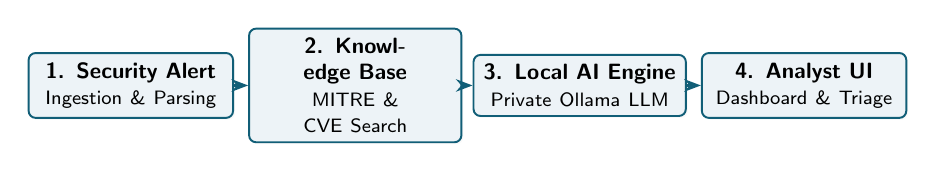
\begin{tikzpicture}[
  font=\sffamily\footnotesize,
  box/.style={rectangle, draw=SOCteal, fill=SOCpale, rounded corners=2.5pt, text centered, inner sep=3.5pt, line width=0.7pt, minimum height=0.72cm, drop shadow={opacity=0.05,shadow xshift=0.7pt,shadow yshift=-0.7pt}},
  arrow/.style={-{Stealth[scale=0.85]}, line width=0.9pt, color=SOCteal}
]
  \node[box, text width=2.35cm] (ingest) at (0,0) {\textbf{1. Security Alert}\\ \scriptsize Ingestion \& Parsing};
  \node[box, text width=2.45cm] (rag) at (2.85,0) {\textbf{2. Knowledge Base}\\ \scriptsize MITRE \& CVE Search};
  \node[box, text width=2.45cm] (llm) at (5.70,0) {\textbf{3. Local AI Engine}\\ \scriptsize Private Ollama LLM};
  \node[box, text width=2.35cm] (ui) at (8.55,0) {\textbf{4. Analyst UI}\\ \scriptsize Dashboard \& Triage};

  \draw[arrow] (ingest) -- (rag);
  \draw[arrow] (rag) -- (llm);
  \draw[arrow] (llm) -- (ui);
\end{tikzpicture}
\end{center}

\vspace{0.05cm}
\begin{columns}[T,onlytextwidth]
\column{0.32\textwidth}
\SOCcard{\linewidth}{Local Ingestion \& DB}{
\begin{itemize}\setlength{\itemsep}{2pt}\footnotesize
  \item Ingests security alerts from systems like Wazuh or Syslog.
  \item Normalizes timestamps, IP addresses, users, and hosts.
  \item Stores records in local PostgreSQL relational database.
\end{itemize}
}

\column{0.32\textwidth}
\SOCcard{\linewidth}{Knowledge Base (Qdrant)}{
\begin{itemize}\setlength{\itemsep}{2pt}\footnotesize
  \item Pre-indexed database containing \textbf{1,762 vector chunks}.
  \item Includes 1,618 MITRE techniques and 144 NVD CVEs.
  \item Finds relevant threat guidance by conceptual similarity.
\end{itemize}
}

\column{0.32\textwidth}
\SOCcard{\linewidth}{Private Local AI (Ollama)}{
\begin{itemize}\setlength{\itemsep}{2pt}\footnotesize
  \item Hosts open-weights 8B model (\texttt{qwen3:8b}) locally.
  \item Zero-temperature execution for consistent, reliable output.
  \item Verifies that cited reference IDs exist before saving.
\end{itemize}
}
\end{columns}
}

% =============================================================================
% SLIDE 4: Technical Approach: How an Alert is Analysed
% =============================================================================
\SOCslide{3. Technical Approach}{Step-by-Step Alert Reasoning with Plain-English Technical Concepts}{
\begin{center}
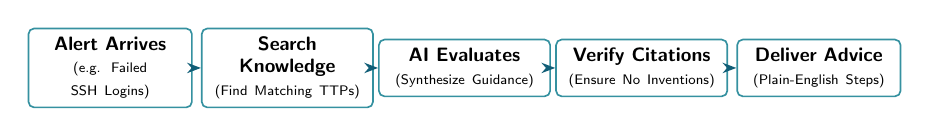
\begin{tikzpicture}[
  font=\sffamily\scriptsize,
  stage/.style={rectangle, draw=SOCtealLight, fill=white, rounded corners=2pt, text centered, inner sep=3.2pt, line width=0.6pt, minimum height=0.52cm},
  arrow/.style={-{Stealth[scale=0.75]}, line width=0.8pt, color=SOCteal}
]
  \node[stage, text width=1.85cm] (s1) at (0,0) {\textbf{Alert Arrives}\\ \tiny (e.g. Failed SSH Logins)};
  \node[stage, text width=1.95cm] (s2) at (2.25,0) {\textbf{Search Knowledge}\\ \tiny (Find Matching TTPs)};
  \node[stage, text width=1.95cm] (s3) at (4.50,0) {\textbf{AI Evaluates}\\ \tiny (Synthesize Guidance)};
  \node[stage, text width=1.95cm] (s4) at (6.75,0) {\textbf{Verify Citations}\\ \tiny (Ensure No Inventions)};
  \node[stage, text width=1.85cm] (s5) at (9.00,0) {\textbf{Deliver Advice}\\ \tiny (Plain-English Steps)};

  \draw[arrow] (s1) -- (s2);
  \draw[arrow] (s2) -- (s3);
  \draw[arrow] (s3) -- (s4);
  \draw[arrow] (s4) -- (s5);
\end{tikzpicture}
\end{center}

\vspace{0.04cm}
\SOCcard{\linewidth}{Plain-English Definitions of Core Concepts}{
\begin{itemize}\setlength{\itemsep}{3pt}\small
  \item \textbf{Retrieval-Augmented Generation (RAG)}: The AI searches a pre-built security knowledge base \textit{before} generating an answer, so its reasoning is grounded in verified documentation rather than memory.
  \item \textbf{Vector Database (Qdrant)}: A specialized database that matches security queries to known threats by conceptual meaning rather than keyword matching alone.
  \item \textbf{Evidence Validation}: An automated check verifying that citation IDs referenced in the AI output match records in the retrieved context before saving results.
  \item \textbf{Local LLM (Ollama)}: An open-weights model executed locally on host hardware, avoiding transmission of internal telemetry to external third-party cloud APIs.
\end{itemize}
}
}

% =============================================================================
% SLIDE 5: Implementation Progress: Frontend & Alert Investigation Walkthrough
% =============================================================================
\SOCslide{2. Implementation Progress}{Frontend Investigation Console: Walkthrough of a Demo Alert}{
\begin{columns}[T,onlytextwidth]
\column{0.48\textwidth}
\begin{tcolorbox}[
  colback=white,colframe=SOCteal,arc=1.5mm,top=3.5pt,bottom=3.5pt,left=4.5pt,right=4.5pt,
  title={\sffamily\bfseries\small Illustrative Synthetic Alert (Evaluation Scenario)},
  coltitle=white,colbacktitle=SOCteal
]
\footnotesize
\textbf{Alert:} SSH Authentication Failure (\texttt{case-01})\\
\textbf{Host:} \texttt{linux-lab (Ubuntu)}\\
\textbf{Source IP:} \texttt{198.51.100.77} \quad\textbar\quad \textbf{User:} \texttt{admin-test}\\
\textbf{Severity:} \colorbox{red!20}{\textcolor{red!80!black}{\textbf{HIGH (Rule Level 10)}}}\\[2.5pt]
\textbf{Observed Telemetry:}\\
\textit{``Failed authentication attempt using non-existent user 'admin-test' from IP 198.51.100.77 on host linux-lab.''}
\end{tcolorbox}

\column{0.48\textwidth}
\begin{tcolorbox}[
  colback=SOCpale,colframe=SOCtealLight,arc=1.5mm,top=3.5pt,bottom=3.5pt,left=4.5pt,right=4.5pt,
  title={\sffamily\bfseries\small AI Assistant Output \& Actionable Guidance},
  coltitle=white,colbacktitle=SOCtealLight
]
\footnotesize
\textbf{Threat Identified:} MITRE ATT\&CK \textbf{T1110 (Brute Force)}.\\[1.5pt]
\textbf{Explanation:} Identifies automated credential guessing targeting user accounts on the SSH service.\\[2pt]
\textbf{Actionable Containment Guidance:}\\
\begin{enumerate}\setlength{\itemsep}{1pt}\scriptsize
  \item Check perimeter firewall rules for source IP \texttt{198.51.100.77}.
  \item Review authentication logs for repeated attempts across accounts.
  \item Enforce public-key authentication and connection rate-limiting.
\end{enumerate}
\vspace{1pt}
\textcolor{SOCgreen}{\textbf{$\checkmark$ Citations Verified:}} Linked to MITRE \texttt{T1110} (ID: 1618).
\end{tcolorbox}
\end{columns}

\vspace{0.08cm}
\SOCbox{\linewidth}{SOCline}{white}{
  \footnotesize\textbf{Workflow Value:} Translates raw event telemetry into structured triage summaries with verified MITRE ATT\&CK references for human analyst verification.
}
}

% =============================================================================
% SLIDE 6: Implementation Progress: Backend, Databases & AI Components
% =============================================================================
\SOCslide{2. Implementation Progress}{Backend Architecture, Databases, and Data-Source Separation}{
\begin{columns}[T,onlytextwidth]
\column{0.48\textwidth}
\SOCcard{\linewidth}{FastAPI Core \& PostgreSQL}{
\begin{itemize}\setlength{\itemsep}{2pt}\small
  \item \textbf{Asynchronous API}: Fast REST backend handling ingestion and real-time trace streaming.
  \item \textbf{PostgreSQL 15+ Store}: Persists 95 alerts, 44 analyses, and 48 evidence links.
  \item \textbf{Schema Versioning}: Alembic migrations ensure reproducible database setup.
\end{itemize}
}

\vspace{0.08cm}
\SOCcard{\linewidth}{Vector Store (Qdrant)}{
\begin{itemize}\setlength{\itemsep}{2pt}\small
  \item \textbf{1,762 Indexed Chunks}: 1,618 MITRE techniques + 144 NVD CVEs.
  \item \textbf{Fast Semantic Search}: Local embeddings retrieve relevant context in under 30 ms.
\end{itemize}
}

\column{0.48\textwidth}
\SOCcard{\linewidth}{Private AI Engine (Ollama)}{
\begin{itemize}\setlength{\itemsep}{2pt}\small
  \item \textbf{Local 8B Model}: Runs \texttt{qwen3:8b} on host machine without external API dependencies.
  \item \textbf{Deterministic Output}: Temperature 0.0 ensures repeatable, auditable reasoning.
\end{itemize}
}

\vspace{0.08cm}
\SOCcard{\linewidth}{Data-Source Isolation \& SIEM}{
\begin{itemize}\setlength{\itemsep}{2pt}\small
  \item \textbf{3 Isolated Modes}: Demo (95 cases), Live Wazuh (empty until connected), Replay.
  \item \textbf{Wazuh Connector}: OpenSearch client implemented; operates in mock mode pending remote deployment.
\end{itemize}
}
\end{columns}
}

% =============================================================================
% SLIDE 7: Testing & Validation
% =============================================================================
\SOCslide{Testing \& Validation}{Rigorous Automated Testing and Citation Integrity Verification}{
\begin{columns}[T,onlytextwidth]
\column{0.48\textwidth}
\SOCcard{\linewidth}{258 Automated Software Tests}{
\begin{itemize}\setlength{\itemsep}{2pt}\footnotesize
  \item \textbf{Backend Suite (Pytest)}: \textcolor{SOCgreen}{\textbf{226 passed}}, 0 failed.
    \begin{itemize}\scriptsize
      \item Ingestion, deduplication, schema normalization.
      \item Vector similarity search and query synthesis.
      \item Tri-mode analysis orchestration and citation checks.
      \item Wazuh transport client and API error handling.
    \end{itemize}
  \item \textbf{Frontend Suite (Vitest)}: \textcolor{SOCgreen}{\textbf{32 passed}}, 0 failed.
    \begin{itemize}\scriptsize
      \item Alert triage console, execution traces, entity graph.
      \item Clean production build compiled in 4.9 seconds.
    \end{itemize}
\end{itemize}
}

\column{0.48\textwidth}
\SOCcard{\linewidth}{Citation Integrity \& System Health}{
\begin{itemize}\setlength{\itemsep}{3pt}\footnotesize
  \item \textbf{100\% Valid Reference Rate}: In completed evaluation records, 100\% of cited evidence IDs existed in the retrieved knowledge set.
  \item \textbf{Scope Qualification}: Validates citation reference existence; does not guarantee that all generated narrative text is factually correct.
  \item \textbf{Live Health Monitoring}: Diagnostic endpoint (\texttt{GET /health}) actively monitors PostgreSQL, Qdrant, and Ollama status.
  \item \textbf{Fault-Tolerant Resumption}: Saves progress per scenario, ensuring zero data loss if benchmarks are interrupted.
\end{itemize}
}
\end{columns}

\vspace{0.04cm}
\SOCbox{\linewidth}{SOCline}{SOCpale}{
  \footnotesize\textbf{Testing Distinction:} Software unit tests (258 passed) confirm code correctness and API stability; threat detection performance is evaluated separately on security benchmarks.
}
}

% =============================================================================
% SLIDE 8: Preliminary Results
% =============================================================================
\SOCslide{4. Preliminary Results}{Findings from Controlled Experiments and Knowledge Base Testing}{
\SOCbox{\linewidth}{SOCbadgeBg}{SOCpale}{
  \footnotesize\textbf{\color{SOCamber}Benchmark Status:} Preliminary evaluation completed on \textbf{12 of 40 scenarios} (36 of 120 planned mode evaluations on Dataset v2); the full benchmark remains ongoing.
}

\vspace{0.03cm}
\begin{columns}[T,onlytextwidth]
\column{0.32\textwidth}
\SOCcard{\linewidth}{Recall@1 ($N=8$ Baseline)}{
\textbf{\large 1.000 vs 0.250}\\[1.5pt]
\scriptsize
Targeted security retrieval found the correct MITRE technique chunk in \textbf{100\% of baseline cases} ($N=8$), versus \textbf{25\%} for basic keyword search.
}

\column{0.32\textwidth}
\SOCcard{\linewidth}{Valid Reference Rate}{
\textbf{\large 100\% Valid}\\[1.5pt]
\scriptsize
Across all 24 completed RAG evaluations on Dataset v2, \textbf{100\% of cited evidence IDs} matched retrieved records, preventing fabricated references.
}

\column{0.32\textwidth}
\SOCcard{\linewidth}{Host Wall Latency}{
\textbf{\large 36.8 s vs 79.6 s}\\[1.5pt]
\scriptsize
Raw LLM inference averaged \textbf{36.8 s} per alert; full evidence-grounded analysis averaged \textbf{79.6 s} on local host hardware without cloud GPUs.
}
\end{columns}

\vspace{0.03cm}
\SOCcard{\linewidth}{Plain-English Interpretation of Results}{
\begin{itemize}\setlength{\itemsep}{1pt}\footnotesize
  \item \textbf{Retrieval Quality vs. Latency}: Targeted threat retrieval consistently supplies the correct MITRE technique to the LLM, but adds retrieval and prompt processing overhead.
  \item \textbf{Preliminary Nature}: Results reflect the initial 12 scenarios; completion of all 40 scenarios is required for final statistical conclusions across threat categories.
\end{itemize}
}
}

% =============================================================================
% SLIDE 9: Limitations & Future Work
% =============================================================================
\SOCslide{Limitations \& Future Work}{Transparent Engineering Constraints and Roadmap for Final Review}{
\begin{columns}[T,onlytextwidth]
\column{0.48\textwidth}
\SOCcard{\linewidth}{Current Engineering Constraints}{
\begin{itemize}\setlength{\itemsep}{2.5pt}\footnotesize
  \item \textbf{Host Memory Limits}: Hosting a full Wazuh cluster alongside the 8B LLM requires >16 GB RAM; currently operates in verified mock mode.
  \item \textbf{Inference Latency}: 35--80s per alert is suitable for deep advisory, but needs acceleration for high-volume queues.
  \item \textbf{Curated Scenarios}: Evaluated on structured attack cases; live enterprise noise validation remains ongoing.
\end{itemize}
}

\column{0.48\textwidth}
\SOCcard{\linewidth}{Milestones for Final Review}{
\begin{itemize}\setlength{\itemsep}{2pt}\footnotesize
  \item \textbf{1. Complete Benchmark}: Run remaining 28 scenarios (84 evaluations) on Dataset v2.
  \item \textbf{2. Remote Live Wazuh}: Connect the verified OpenSearch connector to an external Wazuh cluster.
  \item \textbf{3. Model Optimization}: Test lightweight 3B/4B quantized models to reduce latency under 10s.
  \item \textbf{4. Analyst Feedback}: Add one-click analyst ratings to refine prompt recommendations.
\end{itemize}
}
\end{columns}

\vspace{0.08cm}
\SOCbox{\linewidth}{SOCline}{SOCpale}{
  \footnotesize\textbf{Evidence Transparency:} Claims of live Wazuh integration are withheld until validated on a dedicated remote server; presented results reflect verified local software and retrieval grounding.
}
}

% =============================================================================
% SLIDE 10: Conclusion & Questions
% =============================================================================
\SOCslide{Conclusion}{Summary of Achieved Milestones for PPD-II Second Review}{
\begin{columns}[T,onlytextwidth]
\column{0.53\textwidth}
\SOCcard{\linewidth}{Summary of Deliverables}{
\begin{itemize}\setlength{\itemsep}{3pt}\footnotesize
  \item \textbf{Functional Prototype}: Implemented on-premise advisory assistant integrating FastAPI, PostgreSQL, Qdrant, Ollama, and React 19.
  \item \textbf{Security Knowledge Base}: Pre-indexed 1,762 MITRE ATT\&CK and CVE chunks to ground AI reasoning in real security facts.
  \item \textbf{Verified Code Quality}: 258 automated tests passing (226 backend, 32 frontend) with 0 regressions.
  \item \textbf{Preliminary Findings}: Demonstrated 100\% valid reference rate and strong baseline retrieval accuracy (Recall@1 = 1.0 vs 0.25).
  \item \textbf{Immediate Roadmap}: Complete remaining 84 evaluations and connect remote live SIEM.
\end{itemize}
}

\column{0.44\textwidth}
\begin{tcolorbox}[
  colback=SOCteal,colframe=SOCteal,arc=2mm,center,top=6pt,bottom=6pt,
  drop shadow={opacity=.12,shadow xshift=1pt,shadow yshift=-1pt}
]
  \centering
  \textcolor{white}{\large\bfseries Thank You!}\\[4pt]
  \textcolor{SOCtealLight!40}{\small\textbf{Questions \& Discussion}}\\[8pt]
  \textcolor{white!95}{\footnotesize\textbf{Project Team}}\\[2pt]
  \textcolor{white!85}{\scriptsize Kunal Sanga (2301341031)}\\[1pt]
  \textcolor{white!85}{\scriptsize Soumili Ghosh (231341057)}\\[1pt]
  \textcolor{white!85}{\scriptsize Bivan Jena (2301341021)}\\[5pt]
  \textcolor{white!90}{\scriptsize\textbf{Guide:} Miss Alka Dash}\\[1pt]
  \textcolor{white!70}{\tiny Assistant Professor, Department of CSE}\\[2pt]
  \textcolor{white!60}{\tiny Silicon Institute of Technology, Sambalpur}
\end{tcolorbox}
\end{columns}
}

\end{document}